\subsection{Architecture}

This section aims to give a broad view of the components and how all of them work together to satisfy the needs of our prototype. A more detailed explanation for each component will be discussed in section \ref{sssec:technologies}.

\begin{figure}[t]%evtl:[t] [!htbp]
\centering
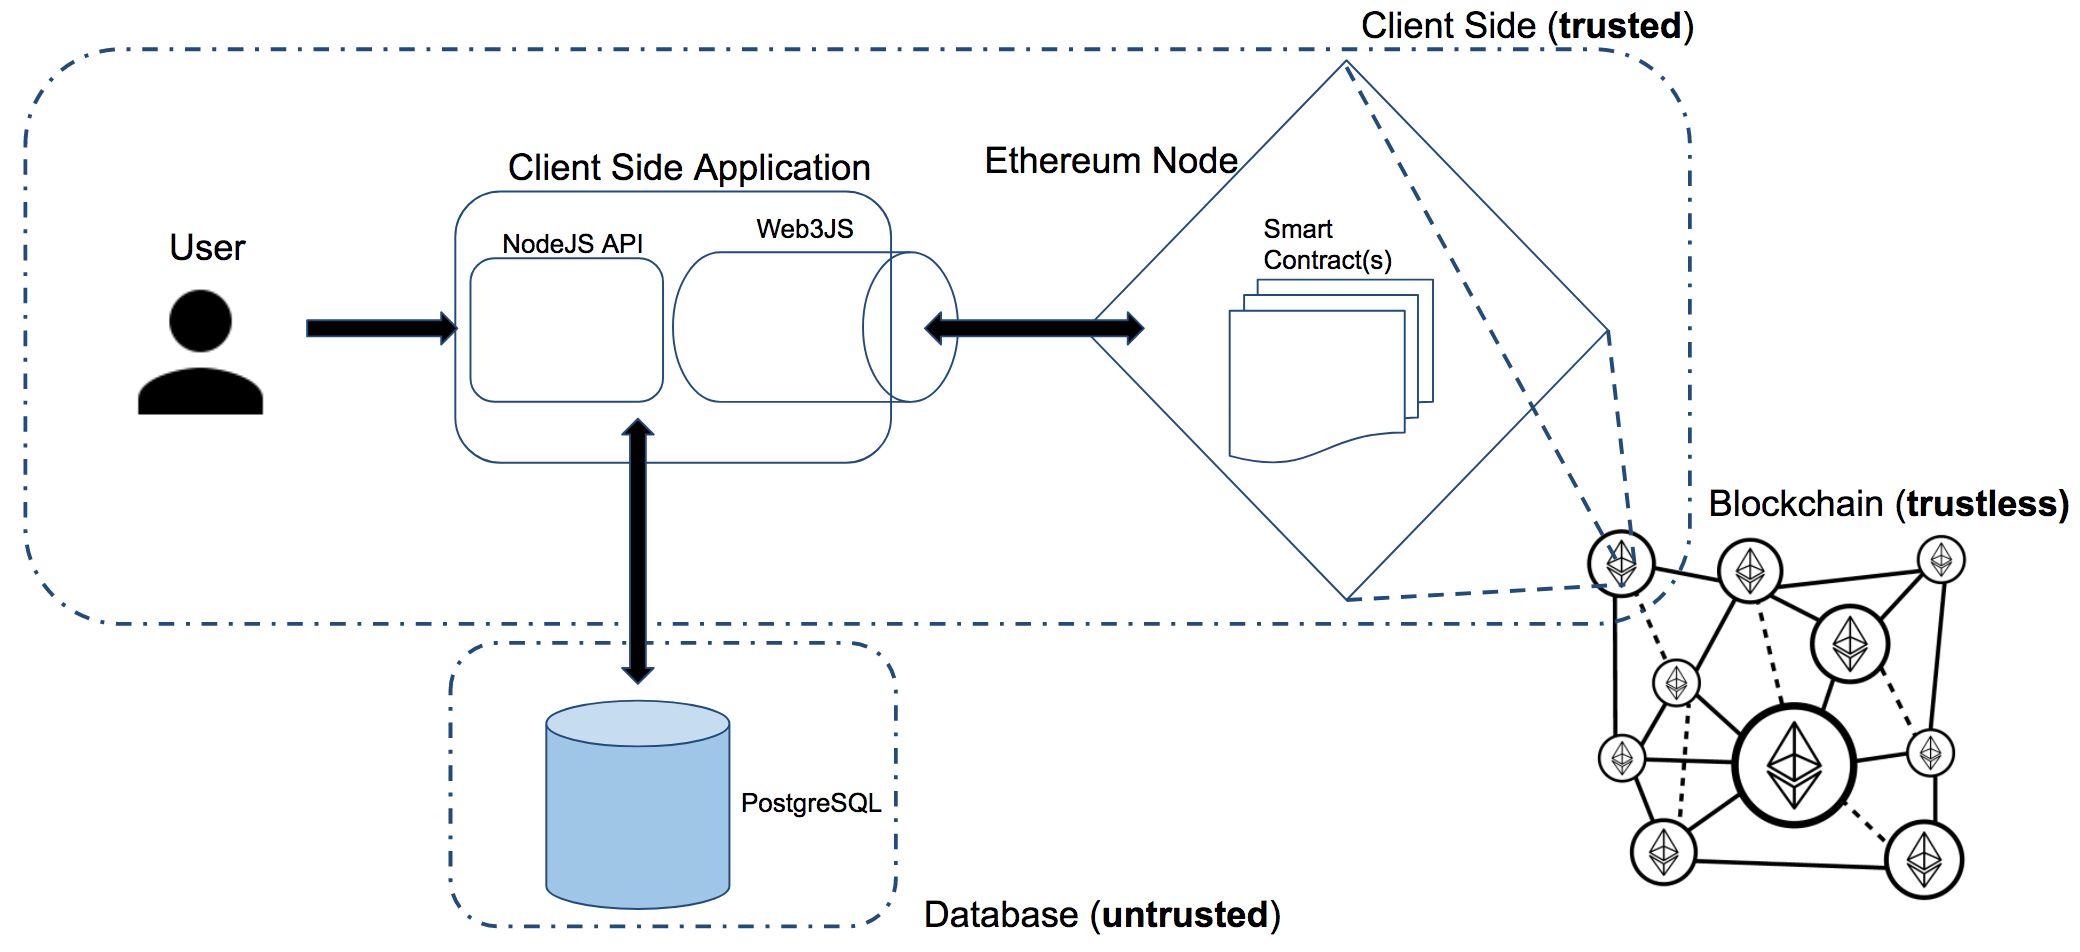
\includegraphics[width=1.0\textwidth]{images/architecture.png}
\caption{\label{fig:architecture}The architecture of the off-chaining approach.}
\end{figure}

As seen in Figure \ref{fig:architecture}, we have divided our architecture into three sides:
\begin{itemize}
\item Client side
\item Database
\item Blockchain environment
\end{itemize}

\subparagraph{Client Side}
The client side consists of the client side application, and the Ethereum node. The client side application is the biggest component as it bridges the database and the smart contract in the Ethereum node. Currently, we put trust into the client side to a certain extent. The extent of trust varies depending on the use case, but nevertheless, a certain level of trust has to exist. For example, upon insertion of new data, before any data goes into the smart contract to be processed, we trust that the client side application will not alter the values. This assumption also acts as a temporary solution to the problem which we have encountered in performing heavy computations inside the smart contract. This assumption has allowed us to take the computational burden from smart contract to the client side application. This problem and solution will be explained in more details in <this section, core implementation stratey>.

\subparagraph{Blockchain Environment}
The blockchain environment is the decentralized network where the smart contract and its local data are going to ultimately live in. The blockchain decentralized network is trustless. But what it truly means is that the trust is distributed amongst all nodes in the network. It also means that we do not enforce an external institution to make sure that the smart contract and its local data are accurate and consistent (integrity). The environment itself ensures the integrity of the data.

\subparagraph{Database}
The database however, is not trusted. Though in our approach we use the database to store data that is going to be used again in the smart contract, we cannot trust the database. The database is prone to internal attacks that can affect the integrity of the data. But at the same time, a database allows us to store large amount of data, and it can be easily integrated with other applications or systems, highly suitable for an off-chaining approach. Hence our approach includes leveraging data integrity check mechanisms when using off-chained data from an untrusted source, such as the database, in the smart contract.

\subparagraph{Transportation Layer}
We have not only made the assumption that our client side is trusted, but also that the transportation layer is secured. Prior to the assumption, we have thought of attacks such as the man-in-the-middle attack, and how detrimental this attack is when we want to save raw data to the database, or when communicating with the smart contract. For example, it could happen that the hashes created in the client side application are altered upon sending them to the smart contract during the initial step. The first step of the approach includes the client side application hashing the raw data and sending the hashes to the smart contract to be stored, mapping the off-chained data to their hashes. Hence, if an attack changes a hash to a different data’s hash, then someone may be able to pass the integrity check by reusing that altered hash’s raw data value.

\subparagraph{Application Flow}
There are two most basic and general approaches in which the user interacts with our client side application. 

\begin{itemize}
\item Inserting a new data
\item Performing a specific action with that data
\end{itemize}

In most general cases, the flow of our application when a user wants to insert a new data goes in the following way: 

\begin{enumerate}
\item User posts a request to client side application with all the data that are required in the specified data model. 
\item Client side application creates a Merkle Tree using the data sent.
\item Client side application sends the Merkle root hash to the the smart contract.
\item smart contract stores the root hash as a local variable.
\item smart contract fires an Event to the client side application to let it know if it has successfully stored it. 
\item Client side application performs a database query to store the data and the root hash into the database.
\item Database stores it.
\item Return success message to the user. 
\end{enumerate}

In most general cases, the flow of our application when a user wants to perform a specific task through the smart contract while using the Off-chained data goes in the following way. 

\begin{enumerate}
\item User creates a request to the client side application to perform a specific smart contract function. 
\item Client side application triggers relevant smart contract function.
\item smart contract triggers an Event to the client side application to retrieve specific data from database. Specific data can be specified by using the root hash stored in smart contract previously.
\item Client side application listens to Event and queries required data from the database.
\item Client side application creates a Merkle tree from the queried data, and creates a Merkle proof.
\item Client side application sends required data and proof to smart contract via function call.
\item smart contract performs integrity check using the proof from client side application.
\item smart contract continues with the original intended task requested by the user when the proof has passed the integrity check. 
\item smart contract computes a new root hash from the new changed value, and stores it.
\item smart contract triggers an Event back to the client side application containing either the results, or an error when the proof does not satisfy the condition of the integrity check. 
\item Client side application listens to Event stores the new root hash and the new changed value into the database. 
\item Client side application finally returns either a success message, or a failure in case of a failed data integrity check. 
\end{enumerate}
